\subsubsection{Quản lý lớp học}
\begin{figure}[H]
    \centering
    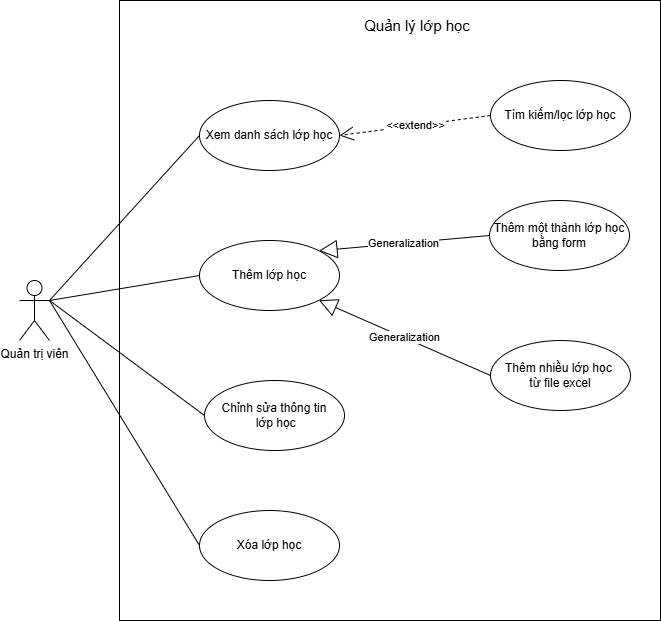
\includegraphics[width=1.0\linewidth]{Images/use-case-diagram/UC02_classes_usecase.drawio.png}
    \vspace{0.3em}
    \caption{UC03 - Quản lý lớp học}
    \label{fig:uc01-usecase}
\end{figure}

% --------------- Bảng use case tổng quát lớp học ----------------
\newpage
\renewcommand{\arraystretch}{1.3}
\begin{longtable}{|m{0.25\textwidth}|m{0.75\textwidth}|}
\hline

\textbf{Use Case Name} 
& \textbf{UC03. Quản lý lớp học} \\ \hline
\endfirsthead

\hline
\textbf{Use Case Name (tiếp)} 
& \textbf{UC03. Quản lý lớp học} \\ \hline
\endhead

\textbf{Actors} 
& Quản trị viên \\ \hline

\textbf{Description} 
& Use case này cho phép quản trị viên thực hiện các thao tác quản lý thông tin lớp học trong hệ thống bao gồm:
\begin{itemize}
    \item Xem danh sách lớp học
    \item Tìm và lọc lớp học
    \item Thực hiện các thao tác thêm, xóa, sửa thông tin lớp học
\end{itemize}
\\ \hline

\textbf{Trigger} 
& Quản trị viên truy cập chức năng quản lý lớp học từ giao diện hệ thống. 
\\ \hline

\textbf{Pre-Conditions} 
& Quản trị viên đã đăng nhập vào hệ thống bằng tài khoản có phân quyền quản lý lớp học. 
\\ \hline

\textbf{Post-Conditions} 
& Thông tin lớp học được hiển thị và cập nhật đúng theo thao tác đã thực hiện. 
\\ \hline

\textbf{Normal Flow} 
& 
\begin{enumerate}
    \item Quản trị viên truy cập module \textit{Quản lý lớp học}.
    \item Hệ thống hiển thị danh sách lớp học.
    \item Quản trị viên chọn một trong các thao tác:
    \begin{itemize}
        \item Xem danh sách lớp học
        \item Tìm và lọc lớp học
        \item Thực hiện các thao tác thêm, xóa, sửa thông tin lớp học
    \end{itemize}
\end{enumerate}
\\ \hline

\textbf{Alternative Flow} 
& Ở bước 3:
\begin{itemize}
    \item \textbf{3a.} Quản trị viên thực hiện tìm kiếm/lọc lớp học, hệ thống hiển thị danh sách lớp học phù hợp với điều kiện tìm kiếm.
\end{itemize}
\\ \hline

\textbf{Exception} 
& Ở bước 1:
\begin{itemize}
    \item \textbf{1a.} Nếu quản trị viên không có phân quyền truy cập vào chức năng quản lý lớp học thì hệ thống sẽ chặn truy cập và không hiển thị module này ở phía giao diện người dùng.
\end{itemize}
\\ \hline
\caption{Bảng mô tả Use Case UC03 - Quản lý lớp học} 
\end{longtable}


